\section{Ontology}
\label{sec:ontology}
% DEBORA
The domain chosen for our ontology is "Organizations". It has been created to answer the provided questions but it is not strongly restricted to them. A domain ontology expresses the links between specific objects and events of that domain through classes (or concepts), properties and attributes of the classes, constraints and instances.
The concepts we want to represent are:
\begin{itemize}
\item The companies.
\item People who play an important role in the company.
\item A nation for people or for the headquarter of a company.
\end{itemize}
The symbols we used to represent this sets are: \textit{Company, Person} and \textit{Nation}.
Then we need symbols to represent the relationships between classes. The relationships we needed are:
\begin{itemize}
\item A person who is the founder of a company.
\item A person who is the CEO of a company.
\item A person who is the CFO of a company.
\item A person who is the Chairman of a company.
\item A person who is the Corporate Officer of a company.
\item A company acquiring a company.
\item The nationality of people.
\item The nation where the headquarter of a company is located.
\end{itemize}
The symbols we used to represent these relationships are: \textit{hasFounder, hasCEO, hasCFO, hasChairman, hasCorporateOfficer, isAcquiredBy, hasNationality} and \textit{hasHeadquarter}. 
The last two are sub-properties of \textit{hasNation} property to solve the ambiguity in deciding if a nationality, for example \textit{italian}, refers to people or companies. Let's look at that in detail:
\begin{itemize}
\item \textit{hasNation} has \textit{"Person \textbf{or} Company"} as domain and \textit{Nation} as range.
\item \textit{hasHeadquarter} has \textit{Company} as domain and \textit{Nation} as range.
\item \textit{hasNationality} has \textit{Person} as domain and \textit{Nation} as range.
\item \textit{Person} is disjoint with \textit{Company}.
\end{itemize}

We also introduced some attribute to classes:
\begin{itemize}
\item The net income of an organization.
\item The market value of a company. For multinational company the market value is referred to the market capitalization. For smaller companies, subsidiaries whose business operations and investments are controlled by the parent corporation, the market value is referred to value at which a company is acquired.
\end{itemize}
The symbols we used to represent these attributes are: \textit{ netIncome} and \textit{marketValue}.
Both the net income and the purchase price are in \textit{billion U.S. dollars}. To note that a billion, in American English, has always equated to a thousand million (i.e. 1'000'000'000).

In order to prevent a computer program to use the symbols '\textit{in the wrong way}' we have introduced  constraints on the way the vocabulary is used:
\begin{itemize}
\item As already mentioned, a person can not be a company and a company can not be a person.
\item People must have at least one nationality. (????????solo una la nazionalità se intesa come nazione di nascita???????)
\item Companies must have at least one headquarter. 
\end{itemize}

The reader can refer to the two file \textit{organizationNotImportedInfer.ttl} and \text
The reader can refer to the files \textit{organization.ttl} and\textit{organizationNotImportedInfer.ttl} in the \textit{data/knowledge} package to see the ontology in detail. The first file is obtained merging the inferred and asserted information of our ontology. The second one contains only the asserted informations.  

Below an entity-relationship model (ER model) for our specific domain of knowledge.
\begin{figure}[H]
\centering
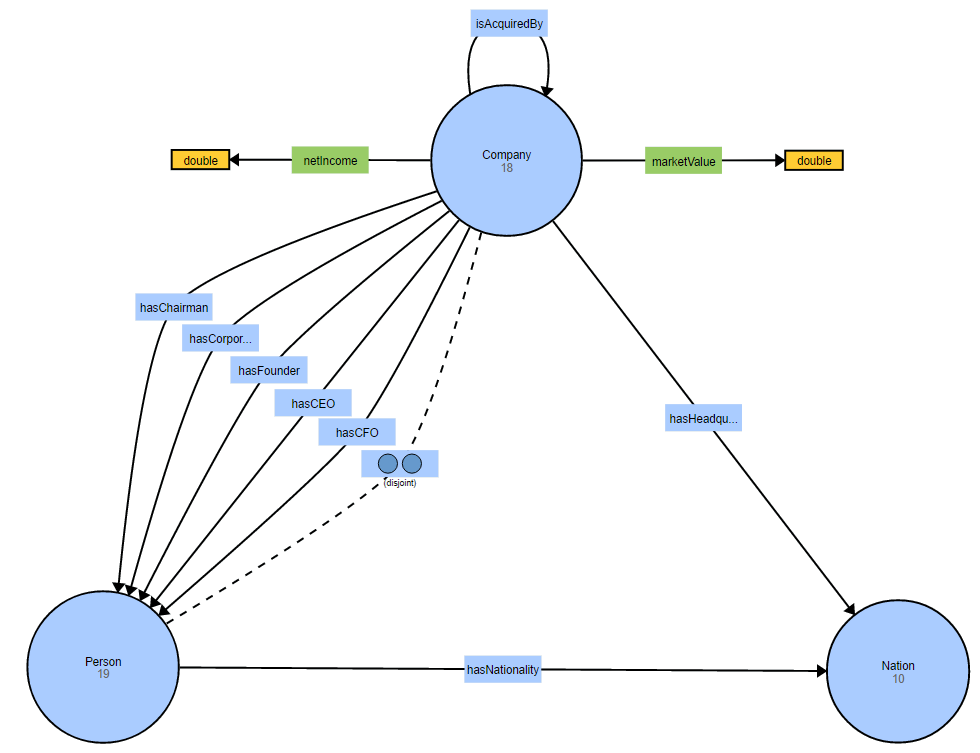
\includegraphics[width=10cm, height=8cm]{fig/ERDiagram.png}
\end{figure}

